\chapter{Background}\label{ch:background}

In the fisrt section, we are going introduce some basics of the design in seL4, then move on to the next section where defines the challenge that we are going to solve in this thesis. Finally, we are going to introduce three related projects, and present how those projects solve the similar problem that we faced in this thesis.     

\section{Overview of seL4}

seL4 has been formally verified for correctness (\cite{Klein_EHACDEEKNSTW_09}) and is the fastest microkernel in the world. The componentized system architecture that seL4 implements enforce the isolation between those untrusted components and other trusted components running on top of the kernel. seL4 was born for safety. The fine-grained capability-based access control model carefully manages the access to the hardware resources from the software components. 

(TODO: Formal descriptio of seL4!)
\subsection{Functionalities in seL4}

(TODO: Cpabilities)

(TODO: Communication and System calls)

(TODO: Memory Management)

(TODO: Scheduling)

The secure and well design of the seL4 microkernel together with the formal verification ensure the kernel itself is robust and is the ideal foundation to build a secure system on top of it (\cite{Klein_AEHCDEEKNSTW_10}). What's more, seL4 is not only secure but also fast. With its performant IPC mechanisms and most advanced mixed critical real-time systems (\cite{Lyons_Heiser_14}) (TODO: use the new paper), seL4 is capable of handling a wide range of real-world scenarios. However, seL4 is relatively young comparing to other mainstream kernels, such as Linux, and its ecosystem is still growing. For those seL4 developers, there are limited tools that can be used while developing seL4 systems. On the other hand, Linux provides us a powerful developing environment with lots of useful tools. Therefore, the main motivation of this project is to explore some ways to leverage the Linux tools in terms of development to make developing seL4 systems much easier and faster.

\section{Challenge}

Developing applications targeted for seL4 in Linux is challenging because seL4 as a microkernel has different semantics and OS model based on seL4 comparing with Linux (In figure \ref{fig:osmodel}).

\begin{figure}[h] (Fixed: fix the bad scaling problem)
    \centering
    \copyrightbox[b]{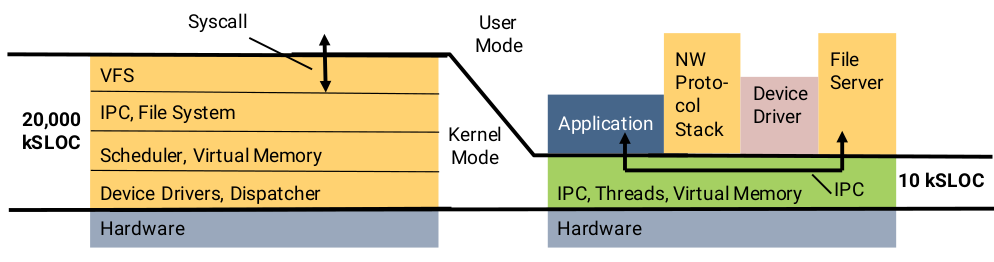
\includegraphics[scale=0.4]{ch2/OS models.png}} % 
    {Source: "The seL4 Microkernel – An Introduction" (p. 3), by Gernot Heiser, 2020, the seL4 foundation. Copyright  under the Creative Commons Attribution-ShareAlike 4.0 International (CC BY-SA 4.0) License.}
    
    \caption{Linux based OS model vs seL4 based OS model.}
    % {\tiny Note: The picture comparison between monolithic OS vs microkernel OS model. Reprinted from "The seL4 Microkernel – An Introduction" (p. 3), by Gernot Heiser, 2020, the seL4 foundation. Copyright  under the Creative Commons Attribution-ShareAlike 4.0 International (CC BY-SA 4.0) License.}
    \label{fig:osmodel}
\end{figure}

Linux is a monolithic kernel that provides a wide range of OS services. The drivers, OS components are implemented inside of the kernel. All those OS services execute in kernel mode. While in seL4, to guarantee the strong isolation of different OS components, seL4 itself is just a thin wrapper of the underlying hardware providing minimal critical services of the hardware resources. The OS services are implemented at the user level as separate components. Such design minimizes the TCB. 

In a monolithic kernel, the user-level applications request the OS services through the system call interfaces that are exported to the user level. A system call will cause a context switch from the user mode to the kernel mode, and the kernel will serve the OS requests by itself. For example, an I/O request from the user level will trigger the system call and the kernel will dispatch such request to the corresponding handler. In Linux, this might be a handler in the VFS layer. Then the VFS layer handler will find the particular file system handler and finally, it will invoke the driver to perform the I/O. After the system call getting triggered, everything happens in the kernel mode until the requests have been served. However, in the seL4 based OS model, it works differently. First, to clarify the term, we are going to call anything that runs in seL4 user level the "seL4 applications". Also, we distinguish those applications into client applications that request OS  services and those server applications that serve the OS services. In the rest of the article, we will use the seL4 applications as the term to make the description easier. When the seL4 client applications request OS services, it will invoke IPC mechanisms provided by the seL4 kernel. (Fixed: description of IPC in seL4) The seL4 IPC is a synchronous method for transmitting small amounts of data and capabilities between seL4 threads. The IPC message passing is the main system call in the seL4, it triggers the context switch to the kernel mode, and the seL4 microkernel will then transport the input to the designated seL4 server application via an exported entry point. Those requests are served by the seL4 server application at the user level. The seL4 client applications and seL4 server applications are isolated components, which ensures the security of the whole system.

As we can see, the main problem here is that seL4 and Linux have different semantics and program flow of serving OS services, the final goal of this project will be providing methods for developing seL4 user-level applications which can either run on Linux or seL4. In other words, we need to provide compatibility between seL4 applications and Linux.

\section{Related Work}

(Fixed: I would expect this to lead off with a discussion on the various abstraction levels we have, and that emulation can happen at each of them)

In this section, we are going to introduce several related projects which provide emulation at different levels from ISA layer to API layer. First, we will present an existing solution to the challenge we stated before, which uses QEMU to provide an ISA-level emulation. Then we will present an API-level emulation project called Cygwin and two ABI-level emulation approaches called Wine and UML. 

\subsection{ISA-level Emulation}

The ISA-level emulation provides a way to run an unmodified target binary code, such as applications or even operating systems like Linux or Windows on a host machine, even if the target's binary code is compiled for targeting a different CPU as the host's. One example of performing ISA-level emulation is using QEMU. 

\subsubsection{QEMU}

(Fixed: This whole section is highly confusing, mangling hardware virtualisation with dynamic translation. This needs much better explanation and classification that these are two completely separate operating modes
Also, the"more efficient" claim is unsubstantiated
Really, this is virtualising at the ISA level, and is just one approach to that)

QEMU is a machine emulator supporting a wide range of ISA and a virtualizer providing us the hardware virtualization feature if the guest's ISA is the same as the host's ISA (\cite{enwikiqemu}). With those features, we are capable of running the seL4 microkernel on top of the Linux, and from the seL4 user-level applications' view, they are still running on top of the seL4 microkernel. 

QEMU is a machine emulator, which means it can use portable dynamic translation to emulate an entire machine, including its processors and peripherals. To convert the guest instruction set into the host instruction set, QEMU will perform two phases. The first phase is the translation and the second phase is the code generation. In the first phase, QEMU splits each target CPU instruction into a few instructions called micro-operations. Each micro-operation is implemented using a small piece of C code that will be compiled by GCC to an object file later. A novel design in QEMU is that QEMU uses dummy code relocations generated by GCC as a place holder with a prefix \emph{$\_\_op\_param$} in the micro-operations, and patches it later when the code generator runs. Because some constants parameters in the target instructions are only known in the runtime. Those relocations can also be references to static data or functions. After that, the \emph{dyngen} will be invoked to generate the dynamic code generator. It will parse the previously generated object file depends on the host operating system's object file format, such as ELF in Linux, to get the symbol table, relocations, and code sections and use that information as the input to generate a dynamic code generator. In the second phase, the dynamic code generator will copy the stream of micro-operations into the host code section and patch the relocations with the runtime parameters. Those relocation patches are host-specific. For optimization, QEMU will maintain a fixed size cache to hold the recently translated blocks of instructions. 

It is flexible in that QEMU can emulate CPUs via dynamic binary translation allowing binary code written for a given ISA to be executed on another ISA, such as running ARM binary on x86. However, the entire system emulation introduces a massive performance overhead. Therefore, QEMU leverages the hardware virtualization extensions,  such as Intel VT-x or AMD-v, which are supported by modern processors to overcome this issue. These technologies directly map a slice of the physical CPU to the virtual CPU. Hence, the instructions of the virtual CPU can directly execute on the physical CPU slice. In Linux, QEMU allows using the KVM as an accelerator to use physical CPU virtualization extensions. However, since KVM is a driver for the physical CPU capabilities, this approach is very tightly associated with the CPU architecture. It means that the benefits of hardware acceleration will be available only if the target system emulated uses the same ISA as the host's and the host processor supports hardware virtualization feature. Otherwise, it won't work.

Although QEMU is an existing solution to emulate the seL4 system in Linux at the ISA layer, it's not an optimal option for emulating a high-performance microkernel like seL4 because of the overhead of hardware virtualization or machine emulation. In the former case, if the guest system such as our seL4 performs a privilege instruction, then it will trigger a world switching to the host, and such overhead is not negligible. In the latter case, if the seL4 system is compiled for targeting a different ISA as our host ISA, then the QEMU will have to perform a full machine emulation and translate the ISA into the host's ISA, which introduces significant overhead. Moreover, though QEMU provides its debugging interfaces to debug the guest system. However, the design goal of QEMU focuses on low-level machine emulation. It's helpful to inspect each instruction's execution of the CPU, but it's hard to use from a high-level seL4 developers' perspective. Because the debugger is not OS aware, the guest OS's context switch might confuse the debugger and lead to a breakpoint missing or a wrong variable value issue. In the following sections, we will introduce other approaches performing emulation at different layers, and then propose approaches used in this thesis to tackle the problem that we stated before in chapter \ref{ch:approaches}.


\subsection{API-level Emulation}

As we mentioned before, the ISA-level emulation involves emulating the emtire machine or using virtualization technologies, which introduces non-negligible overhead. In this section, we will introduce a project which performs emulation approach at the API layer to provide compatibility between two differnt systems.

\subsubsection{Cygwin}

% Cygwin32: A Free Win32 Porting Layer for Unix Applications

The Cygwin is a compatibility layer that allows Unix-like applications to run on top of Windows (\cite{enwikicygwin}). This is achieved by introducing a DLL called cygwin1.dll which acts as an emulation layer providing substantial POSIX system call functionalities providing a Unix semantics. With Cygwin, users can access several standard Unix utilities such as bash, etc.

(TODO: diagram of the architecture)
Cygwin began development in 1995 at Cygnus Solutions. In the project, developers provided interfaces called Cygwin API to add the missing Unix-like functionalities in Win32 API, such as fork, signals, select, etc (\cite{Cygwin}). Cygwin will not magically make any Unix-like application's binary code runnable on top  Windows directly. Executing those Unix-ike applications require the recompilation of the application. The source code can be compiled under the Cygwin and linked with the shared library which implements the POSIX system call semantics using the Win32 APIs and native NT APIs. After executing the application, the Cygwin DLL will be loaded into the application's test region so that it has full access to the whole process. Next, shared memory is created containing the instances of the resources that the shared library can access. Therefore, the OS resources such as file descriptors can be tracked. Besides such shared memory regions, each process also has its resource bookkeeping structures, such as signal masks, PID, etc.

Cygwin has several nice designs to implement the POSIX features in Windows. For example, it handles signals by starting a separate thread from the library for only signal handling purposes. This thread waits for the Windows event used to pass signals to the process, and scan through its signal bitmask to handle the signals appropriately. However such thread resides in the same address space as the executing program, the signal sending function for sending a signal to other processes is wrapped with a mutex, and the signal sending function which sends the signal to itself is wrapped by separate semaphore or event pair to avoid them being interrupted. 

Another example is the implementation of sockets. They are mapped on top of the Winsock. But Unix domain socket is not provided in Windows, so Cygwin implements it with the local IPv4 as the address family. Besides, Cygwin provides the Winsock initialization on the fly, as the Winsock requires to be initialized before the socket function is called. For implementing the POSIX select, Cygwin implements the polling of file handles besides socket type handles by sorting the file descriptors into different types and creating a thread for each type of the file descriptors present to poll those file descriptors with Win32 API. Such a design is because the Winsock only works on socket type file descriptors.

(Fixed: mention somtimes the implementation of the emulation can be complex because of the poor mapping between two systems.)              

The API layer emulation requires to utilize the host systems' functionalities, but it's hard to find an appropriate functions provided by the host systems sometimes. For example, in Unix-like systems, the $fork()$ system call provides a way to create a child process that copies the parent's address space, but there are no appropriate process creation functions in Windows which can be mapped on top of it, so the implementation of $fork()$ in Cygwin is relatively complex.  

Implementing $fork()$ semantics in Windows requiring to copy all of the executable binary and all the DLLs loaded statically or dynamically to be identical as to when the parent process has started or loaded a DLL. This can be problematic as Windows allows the binaries to be renamed to even removed to the recycle bin while the binary is executing, which means they can reside in a different directory or have a different file name. However, an executing process has to access to the binary files via the original filenames to fork its child processes. The solution to this problem is that Cygwin will try to create a private directory that contains the hardlink to the original files and remove it when no process is using it. When the parent process wants to fork a child process, it will first initialize a space in Cygwin process table for the child and create a suspended child process using Win32 CreateProcess system call. 

After that, the parent process will use setjump to save the context and set a pointer to the current context in the Cygwin shared memory, and fill the child process's .data and .bss section with its own address space. Next, the parent process will block on a mutex and the child process will run and use the longjump to jump to the saved jump buffer. Then child process will release the mutex that the parent is blocked on and waits for another mutex. The parent process will copy its stack and heap into the child process space then release the mutex that the child is blocking on and return from the fork call. Finally, the child process will wake up and recreates any memory-mapped areas that passed to it and return from the fork call. However, such implementation is not perfectly reliable as in Windows, Windows implements the ASLR starting from Vista, which means the stack, heap, text, and other regions may be placed in different places in each process. This behavior interferes with the POSIX fork's semantic that is the child process has the same address space as the parent process. In that case, Cygwin will try to compensate the movable memory regions at the wrong place but can't do anything with those unmovable regions such as the memory heap.

In summary, adding compatibility at the API layer can solve most of the problems when attempting to run applications from foreign systems. While the downside is that, apparently this will only work when the user of Cygwin can obtain the source code of the application. Meanwhile, it's very difficult to implement every POSIX system call in Windows correctly due to the huge difference between the internal design and the semantics. 

Even though Cygwin is used to make Unix-like applications compatible with the Windows environment, we can still leverage the nice idea that Cygwin uses. To emulate seL4 in Linux we can link applications to a specific library that remaps the system calls with the underlying host's system calls.

\subsection{ABI-level Emulation}

In the previous section, we have introduced Cygwin,which is an API-compatible solution for providing compatibility between Windows and Linux. However, the downside is that it's not binary compatible as we have to obtain the source code first and recompile it. In that case,  if we can't obtain the source code or the application that we want to emulate directly invokes functions via a foreign system's ABI, then it's impossible to perform the emulation. Hence, in this section, we will introduce two ABI-level emulations which are binary compatible.

\subsubsection{Wine}

% https://en.wikipedia.org/wiki/Wine_(software)#Basic_architecture
(TODO: Need to be improved, add more internals related to Wine)

First example that provides the compatibility layer to run Windows applications in Unix-like operating systems is called Wine (\cite{enwikiWine}). However, Wine doesn't emulate the internal Windows logic like a virtual machine or an emulator. Instead, it directly translates the Windows ABI into POSIX-compliant calls. Besides, Wine also provides various Windows services through Wineserver as well as other Windows components. In Wine's architecture, it implements Windows's ABI entirely in the user space, rather than a kernel module. 

A system call from a Windows application usually invokes a particular DLL library, which in turn invokes the user-mode GDI/user32 libraries, and then finally invokes the system calls via Win32 subsystem. However, since the architecture of Windows OS is a hybrid model of monolithic kernel combined with the microkernel, some OS services run as separate processes, so applications need to invoke RPCs to communicate the user-mode services. In that case, this is somehow similar to how seL4 applications request OS services. Although Wine implements the Wineserver to provide services that are provided by the Windows kernel, as well as other OS functionalities, it's impossible to implement all the aspects of the Windows kernel as well as to use native Windows drivers due to the internal architecture of Wine. 

In Wine's architecture, the critical libraries are implemented using shared libraries and loaded dynamically at runtime, while in the seL4 system, all the binary codes are statically linked. So we can't imitate Wine's architecture and implementation. However, with a similar idea as the Wine project, we can still target the emulation layer of seL4 applications at the kernel ABI layer to achieve binary compatibility.

\subsubsection{User-mode Linux}

(TODO: This whole section suffers from being written bottom-up (or bottom-down?) rather than to-down. There's no big-picture view, no abstractions, just a collection of seemingly random detail. Iris totally impenetrable by someone who doesn't have a lot of OS Ann's Linux background )

UML is an old project used to port a Linux kernel to the userspace. This can be helpful to the system developers as it provides a nice way to develop and debug the kernel as well as to make several interesting applications possible for Linux (\cite{JD06}). 

In UML's architecture, it treats Linux as a platform to which the kernel can be ported. All the implementation fully leverages the Linux system calls without any modification of the host kernel. And all the user-level code can run natively on the processors without any instruction emulation overhead. The implementation creates a separate thread that uses the $ptrace()$ system call to trace all the other threads running in UML. 

(TODO: explain the how to the tracing thread control the context switch)

\subsubsection{System Call}

(TODO: Diagram)
Since the transition between user mode and the kernel mode is controlled by the tracing thread, it will intercept all the signals and system calls that the running process issues and then transit from the user mode to the kernel mode and continue executing the particular process without tracing it. (TODO: add constraint that this happens in the emulated mode) The distinction of the user mode and the kernel mode is whether the process is being traced by the tracing thread. After changing the register which contains the syscall number into the syscall number for $getpid()$ and restoring a previously saved thread registers state, the tracing thread will invoke the syscall handler to accomplish the syscall request, then finally return the process to the user mode. 

\subsubsection{Trap and Fault}

(TODO: Diagram)
UML not only virtualizes system calls but also implements several other Linux OS services and functionalities. For example, to handle the processor traps or faults, it implements those with signals and installs handlers for each. Once the tracing thread captures the signals that the process received, it will switch to the kernel mode and continue executing the process in the handler.

For the memory fault, UML implements with the $SIGSEGV$ and invokes the handler to figure out whether the fault was because of legal access to an unmapped page or illegal memory access. 

\subsubsection{Interrupt}

(TODO: Explain what those signals are. As the reader won't know)

UML also implements external interrupts and timer interrupts using $SIGIO$ and $SIGALARM$ or $SIGVTALARM$ depending on whether the interrupted process is idling or not. For the external interrupts, it uses $select$ to check which file descriptor has received input then invokes the IRQ handler. For the timer interrupt, UML also treats it similarly to treating the external interrupt and invokes the particular IRQ handler. 

\subsubsection{Scheduling}

(TODO: explain it well instead of just mention as an overview)

For process scheduling, UML implements scheduling processes by stoping an outgoing one and running an ingoing one as each process has its thread belongs to it. Since each process has its own address space, UML also manages the page mapping of each process as well as the $SIGIO$ queued in each process.

\subsubsection{Virtual memory}

In UML, the kernel and process's virtual memory is implemented as a physical memory-sized file mapping into their address spaces. However, some regions in the address space will be reserved by placing kernel code and data which is unusable.

\subsubsection{Host filesystem access}

UML also implements a virtual file system called $hostfs$ which translates the directly into the functions in the host's $libc$. Hence, it provides direct access to the host filesystem.

UML was a nice project showing a novel way to use Linux interfaces to implement itself, also it demonstrated that porting a kernel in the userspace can be beneficial to both kernel and application development.

From this project's perspective, UML gives us the hint of how to leverage $ptrace$ to intercept the system call from the process being traced as well as how to simulate the kernel in the userspace.




